%%% Local Variables:
%%% mode: latex
%%% TeX-master: t
%%% End:
\documentclass{beamer}
\usepackage[utf8]{inputenc}
\usepackage{graphics}
\usepackage{listings}
\usepackage{caption}

\captionsetup{font=scriptsize,labelfont=scriptsize}

\usetheme{default}
\usecolortheme{rose}

\DeclareGraphicsRule{.pdftex}{pdf}{.pdftex}{}

% \lstdefinelanguage{cfengine}
%   {morekeywords={import,classes,control,admit,copy,editfiles,processes,shellcommands},
%    sensitive=false,
%    morecommment[l]{//},
%   }

\newcommand\Fontvi{\fontsize{6}{7.2}\selectfont}

\lstset{
basicstyle=\tiny,
stringstyle=\tiny,
numbers=left,
numberstyle=\tiny,
stepnumber=2,
frame=single,
%language=cfengine,
captionpos=b
}

\title{Continuously deliver your puppet code with jenkins, r10k and git\\}
\author{Toni Schmidbauer}

\begin{document}

\begin{frame}
  \center
\includegraphics[height=2.5cm,width=7cm]{../pics/puppetcamp_300dpi}
  \titlepage
\end{frame}

\begin{frame}
  \frametitle{whoami}
  \begin{itemize}
  \item SysAdmin@s-itsolutions.at
  \item toni@stderr.at
  \item stderr@jabber.org
  \item \url{http://stderr.at}
  \item \url{http://github.com/tosmi}
  \end{itemize}
\end{frame}
\begin{frame}

  \frametitle{Agenda}

  \begin{itemize}
  \item A short story about configuration managment
  \item What is continuous delivery
  \item Tools used to achieve continuous delivery
  \item DEMO
  \item Things to improve
  \end{itemize}

\end{frame}

\begin{frame}
  \frametitle{A short story about configuration management (CM)}

  \begin{itemize}
  \item<1-> We manage a very diverse environment of UNIX/Linux Systems (Solaris 10/11, AIX, RHEL/CentOS 5/6/7)
  \item<2-> Before CM we had \textbf{strict} standards on how to manage these systems
  \item<3-> The problem: \\count(teammembers) == count(standards)
  \item<4-> So configuration management is the solution to all our problems
  \end{itemize}

\end{frame}

\begin{frame}
  \frametitle{The solution to all our problems}
  \pause
  \begin{itemize}
  \item Broke our systems
  \end{itemize}
\end{frame}

\begin{frame}
  \center{\huge{WHY????}}
\end{frame}

\begin{frame}
  \frametitle{Problems with our old CM system}

  \begin{itemize}
  \item <1-> Deployments sucked
    \begin{itemize}
    \item <2-> Deployment via manual tagging and checkout, so mistakes happened
    \item <2-> Deployment in stages, but we always had to cross our fingers
    \end{itemize}
  \item <3-> Testing sucked
    \pause
    \begin{itemize}
    \item <4-> No Unittest
    \item <4-> No acceptance tests
    \end{itemize}
  \item <5-> No immediate feedback if things where ok or \textbf{not}
  \item <6-> Systems installed without CM are hard to bring under CM control
  \item <7-> Every system was a special case
  \end{itemize}
\end{frame}

\begin{frame}
  \center{\huge{So whats our solution?}}
\end{frame}


\begin{frame}
  \frametitle{Continuous delivery}
  \begin{itemize}
  \item<1-> is a pattern for getting software from development to release
  \item<2-> this pattern is called \textbf{the deployment pipeline}
  \end{itemize}
  \footnote{Continuous Delivery: Jez Humble, David Farley}
\end{frame}

\begin{frame}
  \frametitle{The deployment pipeline}
  \begin{figure}[ht]
    \centering
      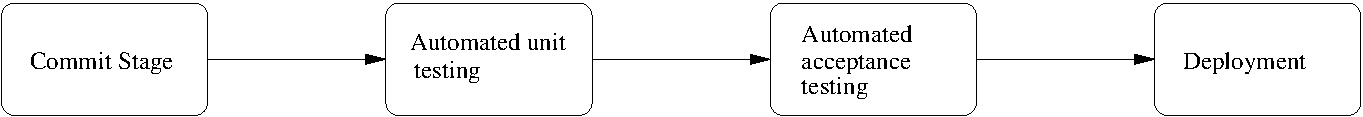
\includegraphics[height=1.2cm,width=11.5cm]{../pics/deployment_pipline}
    \label{fig:stack}
  \end{figure}
\end{frame}

\begin{frame}
  \begin{figure}[ht]
    \centering
      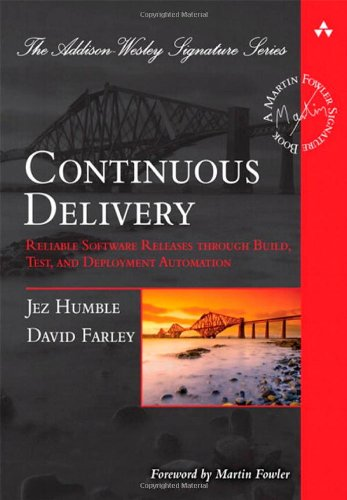
\includegraphics[height=7.5cm,width=6cm]{../pics/cd_book}
    \label{fig:stack}
  \end{figure}
\end{frame}

\section{Tools we used to build a deployment pipeline}
\begin{frame}
  \center \huge Tools to build a deployment pipeline
\end{frame}


\begin{frame}
  \frametitle{Jenkins}

  \begin{itemize}
  \item Jenkins is an Open Source continuous integration server
  \item It's purpose is to execute and monitor jobs
  \item Jobs are shell scripts or any other thing that's executable
    and returns 0 on success
  \item You can link jobs together, thats our pipeline
  \item Many plugins available to extend Jenkins (e.g. git, build-pipeline, monitor)
  \end{itemize}

\end{frame}


\begin{frame}
  \frametitle{Jenkins II}
  \begin{figure}[ht]
    \centering
      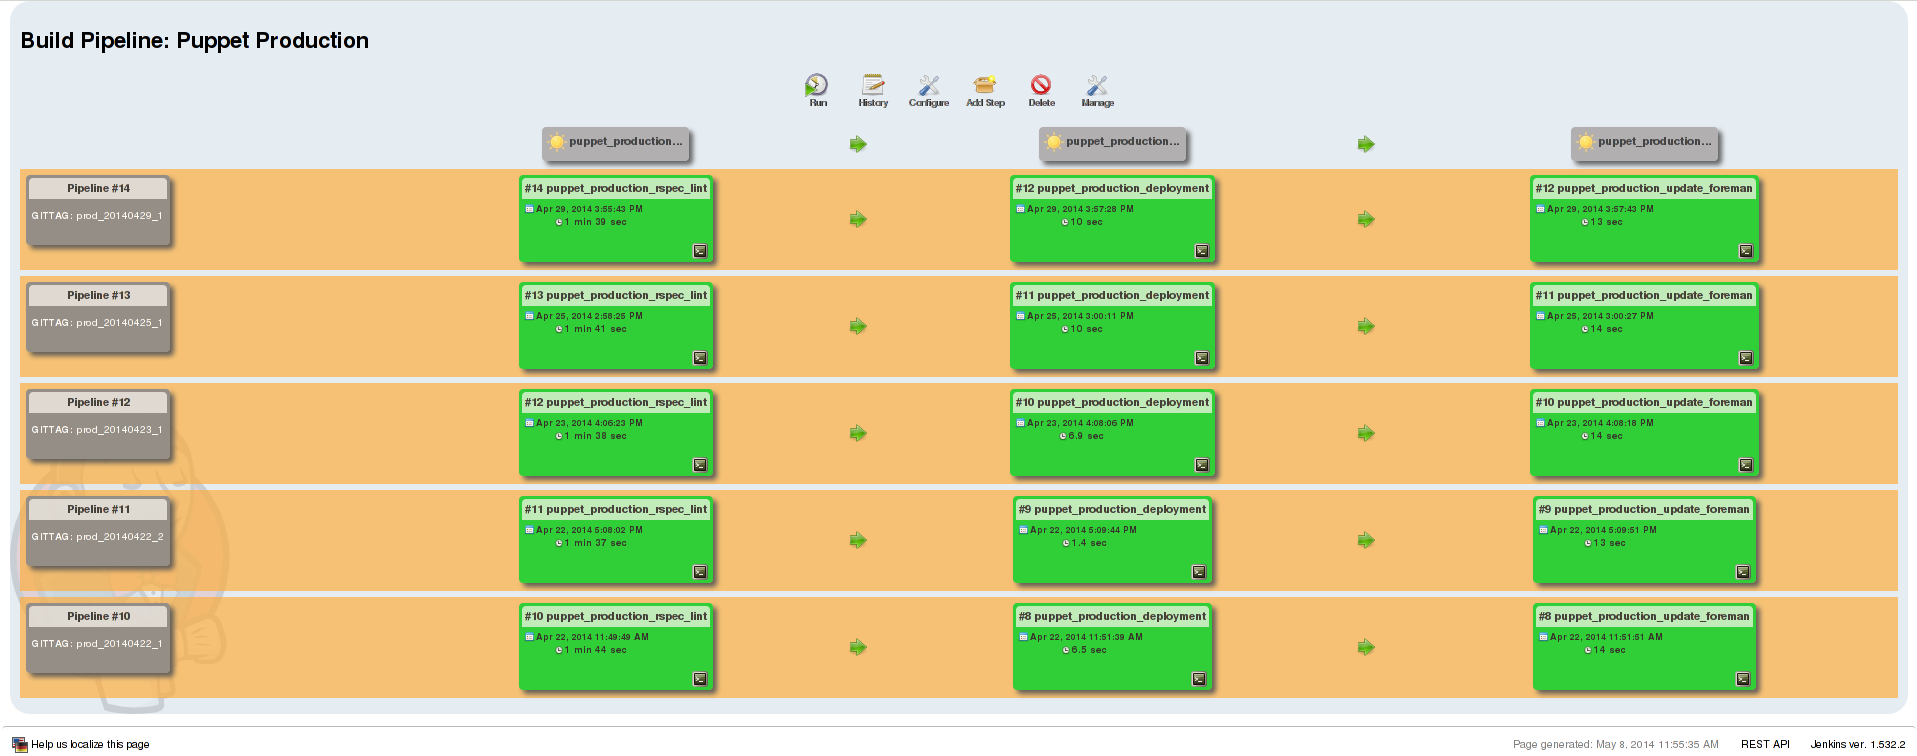
\includegraphics[height=3.5cm,width=11.5cm]{../pics/jenkins_pipeline}
    \label{fig:stack}
  \end{figure}
\end{frame}


\begin{frame}
  \frametitle{Monitoring with Jenkins}
  \begin{figure}[ht]
    \centering
      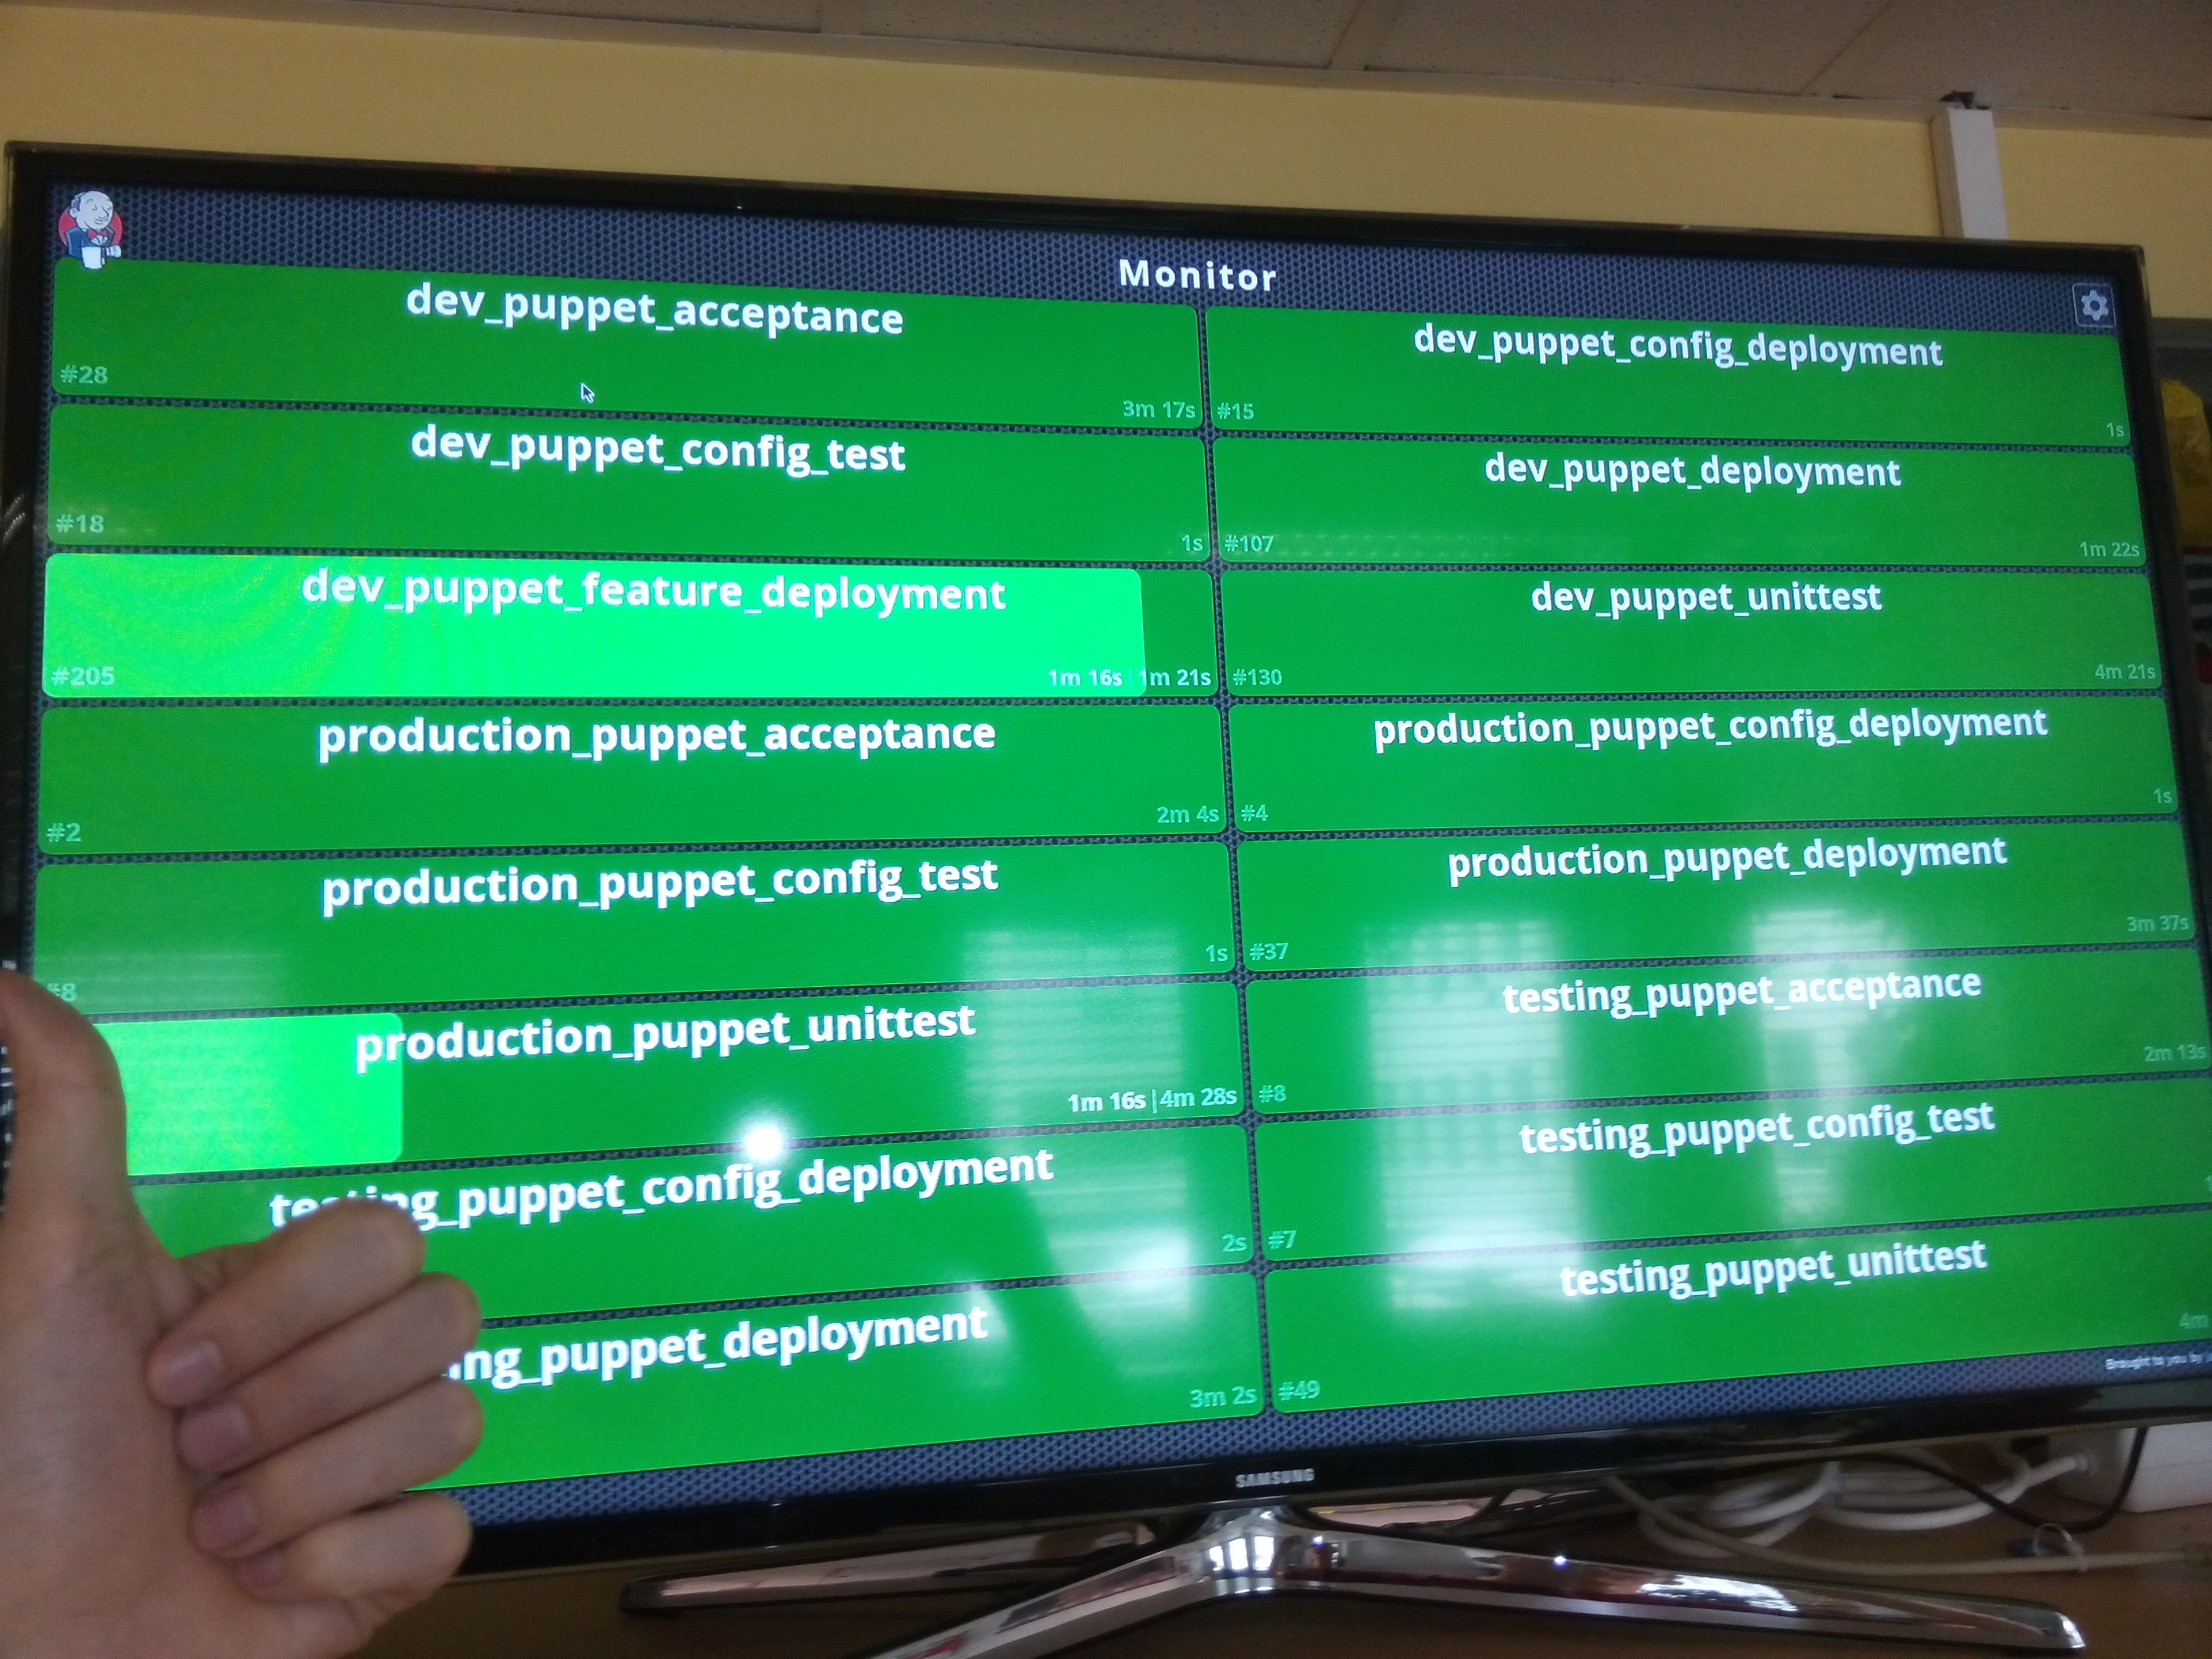
\includegraphics[height=6cm,width=11cm]{../pics/jenkins_monitor_live}
    \label{fig:stack}
  \end{figure}
\end{frame}

\begin{frame}
  \frametitle{GIT}

  \begin{itemize}
  \item \textbf{git push} triggers the deployment pipeline
  \item One central repository managed with gitolite (access control
    for git) for internal modules
  \item 3 main branches
    \begin{itemize}
    \item development
    \item testing
    \item production
    \end{itemize}
  \item feature branches for new site local modules
  \item hiera data is in the same repository
  \end{itemize}
\end{frame}

\begin{frame}
  \frametitle{GIT repository layout}

  \begin{itemize}
  \item \texttt{modules/}:
    \begin{itemize}
    \item where r10k stores external (forge, github) modules
    \end{itemize}
  \item \texttt{site/}:
    \begin{itemize}
    \item site local modules, that we do not want to share
    \end{itemize}
  \item \texttt{hiera/}:
    \begin{itemize}
    \item our hiera yaml files
    \end{itemize}
  \item \texttt{Puppetfile}:
    \begin{itemize}
    \item config file for r10k that specifies which external modules we need
    \end{itemize}
  \end{itemize}
\end{frame}


\begin{frame}
  \frametitle{GIT workflow}
  \begin{figure}
    \centering
      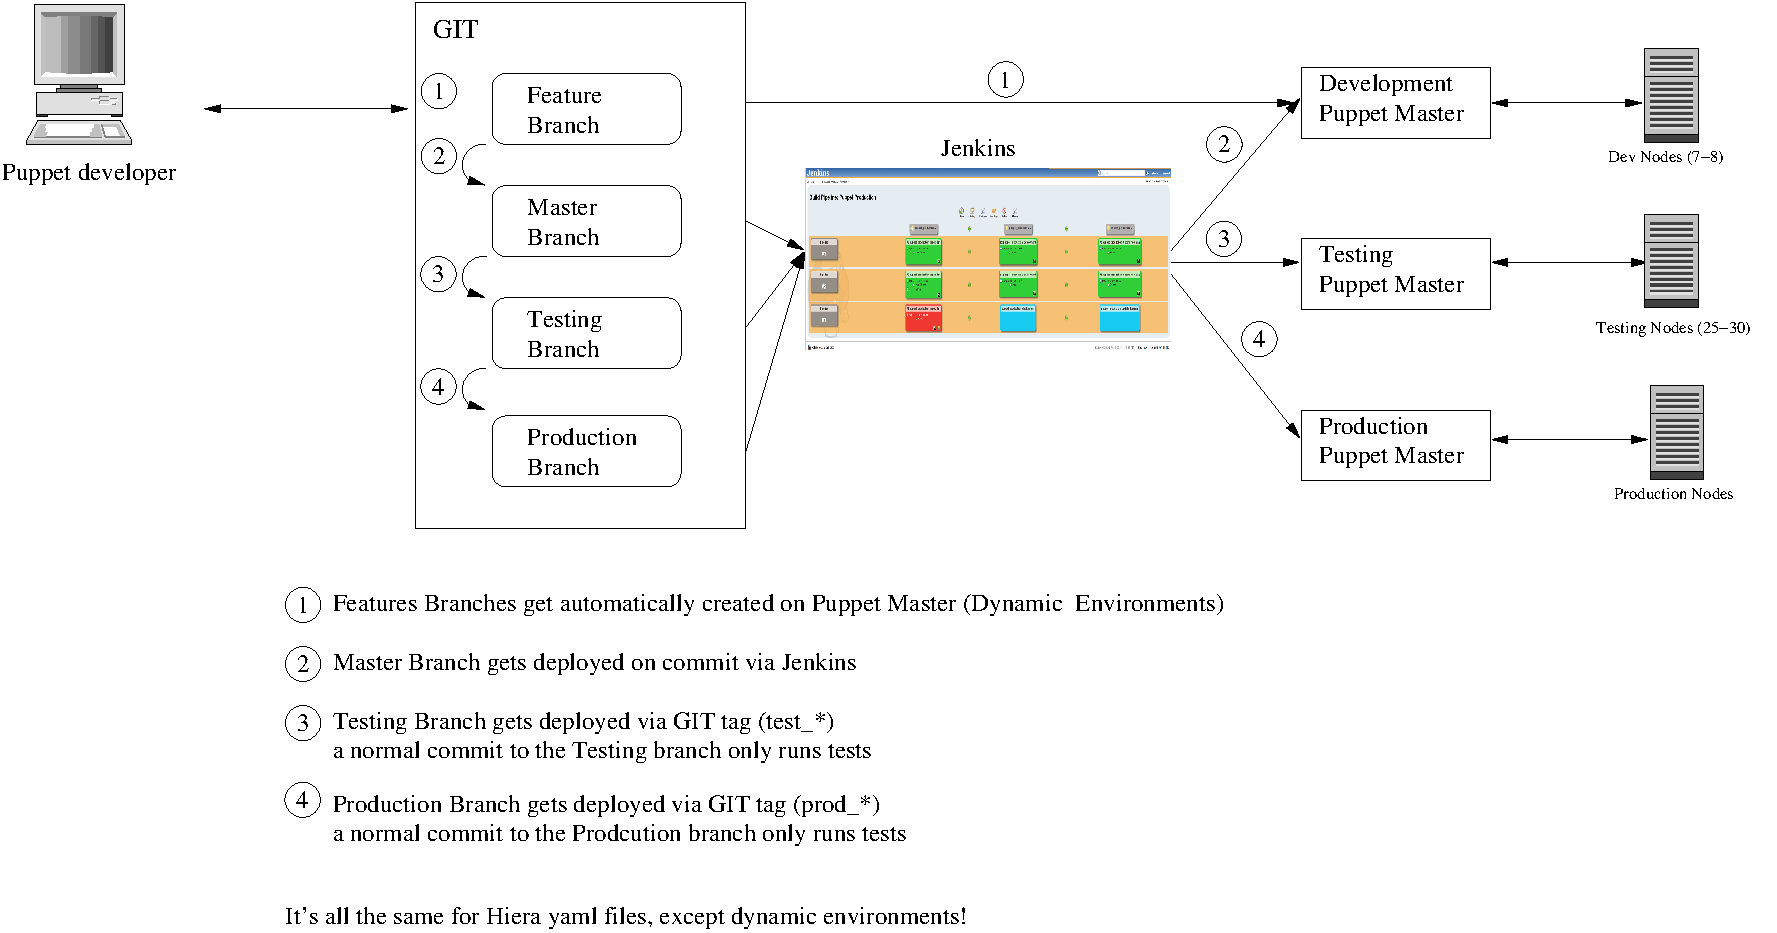
\includegraphics[height=6cm,width=11cm]{../pics/puppet_deployment2}
    \label{fig:stack}
  \end{figure}

\end{frame}

\begin{frame}
  \frametitle{r10k}

  \begin{itemize}
  \item a tool to deploy puppet environments and modules
  \item every git branch gets deploy to a puppet environment
  \item in the current version (1.3.2) dependencies have to be managed
    manually
  \end{itemize}
\end{frame}

  \begin{frame}[fragile]
    \frametitle{Example Puppetfile}
\begin{lstlisting}
forge 'forge.puppetlabs.com'

mod 'puppetlabs/ntp', '3.1.2'
mod 'puppetlabs/postgresql', '3.4.2'
mod 'puppetlabs/stdlib', '4.3.2'
mod 'puppetlabs/firewall', '1.1.3'
mod 'puppetlabs/apache', '1.1.1'
mod 'puppetlabs/lvm', '0.3.2'
mod 'nosolutions/tsm', '0.2.2'
mod 'saz/sudo', '3.0.6'
mod 'spiette/selinux', '0.5.4'

mod 'concat',
    :git => 'https://github.com/puppetlabs/puppetlabs-concat',
    :commit => 'feba3096c99502219043b8161bde299ba65e7b8a'
\end{lstlisting}

    You are able to pin to a git tag / branch / commit hash

\end{frame}

\begin{frame}
  \frametitle{a word on testing}

  \begin{itemize}
  \item you must have unit tests for your puppet code: \textbf{rspec-puppet}
  \item for acceptance tests there's puppetlabs/beaker
  \item you need to test everything to get most out of the build
    pipeline
  \item we test
    \begin{itemize}
    \item interal puppet modules
    \item hiera data
    \item puppet configuration
    \item all internal modules are required to have rspec tests
    \end{itemize}
  \end{itemize}
\end{frame}

\begin{frame}[fragile,fragile]
  \frametitle{rspec-puppet}

  samplemodule/manifests/init.pp

\begin{lstlisting}
class samplemodule ( $message = 'defaultmessage' ) {
  notify { 'samplemessage':
    message => "This is the sample module, my message is: $message",
  }
}
\end{lstlisting}

  samplemodule/spec/classes/samplemodules\_spec.rb

  \begin{lstlisting}
require 'spec_helper'

describe 'samplemodule', :type => :class do
  context 'with default parameters' do
    it { should contain_notify('samplemessage') }
  end
end
  \end{lstlisting}

\end{frame}

\begin{frame}
  \center{\huge DEMO}
\end{frame}

\begin{frame}
  \frametitle{Things to improve}

  \begin{itemize}
  \item We need more test Systems (Centos/RHEL/Solaris)
  \item We need more acceptance tests
  \item Puppetlabs should package beaker as a rpm/deb whatever, gems
    suck in production
  \end{itemize}
\end{frame}

\begin{frame}
  \center{\huge Thanks for you attention!}
\end{frame}

\end{document}
